\documentclass[italian]{beamer}

%%% Dichiarazione dei pacchetti standard.
\usepackage[utf8x]{inputenc}
\usepackage{graphicx}    % inclusione graph images (eps)
\usepackage{multirow}
\usepackage{booktabs}
\usepackage{units}
\usepackage{url}
\usepackage{lmodern}
\usepackage{pstricks}
\include{pst-plot}
\include{pst-3d}
\setbeamertemplate{navigation symbols}{\insertframenumber} 

\usetheme{Frankfurt}
\usecolortheme{wolverine}

\newcommand{\qmo}{``}
\newcommand{\qmc}{''}
\newcommand{\meson}[1]{\ensuremath{\mathrm{#1}}}
\newcommand{\ptrel}{\ensuremath{p_{t}^{\text{rel}}}}
\graphicspath{{images/}}

%%% Titolo e autore.
\title[Studi preliminari per la misura del mixing a CMS]{Studi preliminari per la misura del mixing a CMS}
\author{Matteo Abis}
\institute{Università di Padova}
\date{\today}

\begin{document}

\begin{frame}
    \titlepage
\end{frame}

\begin{frame}
    \frametitle{Oscillazione di mesoni B}
    \begin{block}{Oscillazione o \emph{mixing}}
        {trasformazione spontanea dei mesoni B nella propria
        antiparticella}
    \end{block}
    \begin{figure}[h]
        \centering
        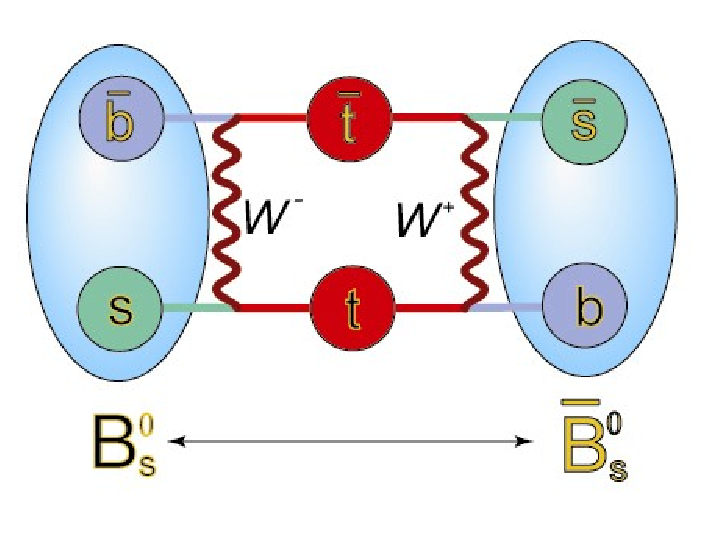
\includegraphics[width=.3\textwidth]{BsMixingBox.eps}
    \end{figure}
    test molto sensibile del modello standard.
\end{frame}

\begin{frame}
    \frametitle{Misura della frequenza di oscillazione}
    \begin{itemize}
        \item produzione di coppie $\meson{B}\meson{\bar{B}}$;
        \item osservazione di stati finali leptonici;
            \begin{itemize}
                \item nessuna oscillazione $\longrightarrow$ stato finale
                    $\mu^+\mu^-$;
                \item oscillazione $\longrightarrow$ stato finale
                    $\mu^+\mu^+$ o $\mu^-\mu^-$.
            \end{itemize}
    \end{itemize}
\end{frame}

\begin{frame}
    \frametitle{Identificazione dei $\mu$ da B}

    Selezioni per i $\mu$:
    \begin{itemize}
        \item all'interno di \emph{jet}.
        \item traccia nel \emph{tracker} e nelle camere a $\mu$;
        \item $p_t > \unit[3]{GeV/c}$;
        \item $|\eta| < 2.1$;
        \item almeno 12 \emph{hit} nel rivelatore;
        \item almeno un \emph{hit} nella parte più interna (\emph{pixel});
        \item $\chi^2 / \text{NDF} < 10$.
    \end{itemize}

    Selezioni per i \emph{jet}:
    \begin{itemize}
        \item $p_t > \unit[10]{GeV/c}$;
        \item $|\eta| < 2.1$.
    \end{itemize}
\end{frame}

\begin{frame}
    \frametitle{Prima fase}
    \framesubtitle{Scrematura dei dati di CMS}

    Dati dei run del 2010\\
    6000000 di eventi $\longrightarrow$ $\sim500000$ eventi interessanti
    \vspace{\baselineskip}\\
    $\sim130000$ eventi simulati
\end{frame}

\begin{frame}
    \frametitle{Seconda fase}
    \framesubtitle{Analisi dei fondi}

    \begin{description}
        \item[segnale: ]$\mu$ da decadimenti del mesone $\meson{B}$;
        \item[fondo: ] decadimenti indiretti $b \rightarrow c \rightarrow
            \mu$, decadimenti di $c$, pioni, etc.
    \end{description}

    Discriminazione:\\
    i $\mu$ del segnale tendono ad essere più energetici.
\end{frame}

\begin{frame}
    \frametitle{Misura del momento dei $\mu$}
    \framesubtitle{Definizione del $\ptrel$}

    Sistema di riferimento del quark $b$ che ha prodotto il \emph{jet}\\
    $\rightarrow$ impossibile da calcolare.
    \vspace{\baselineskip}\\

    \begin{block}
        {momento trasverso relativo --- $\ptrel$}
        Proiezione del momento del muone nel piano ortogonale alla direzione
        del \emph{jet}. Non è affetto da \emph{boost} di Lorentz.
    \end{block}
\end{frame}

\begin{frame}
    \frametitle{Spettro di \ptrel}
    \begin{columns}
        \begin{column}{.5\textwidth}
            \centering
            segnale
            \begin{figure}[h]
                \centering
                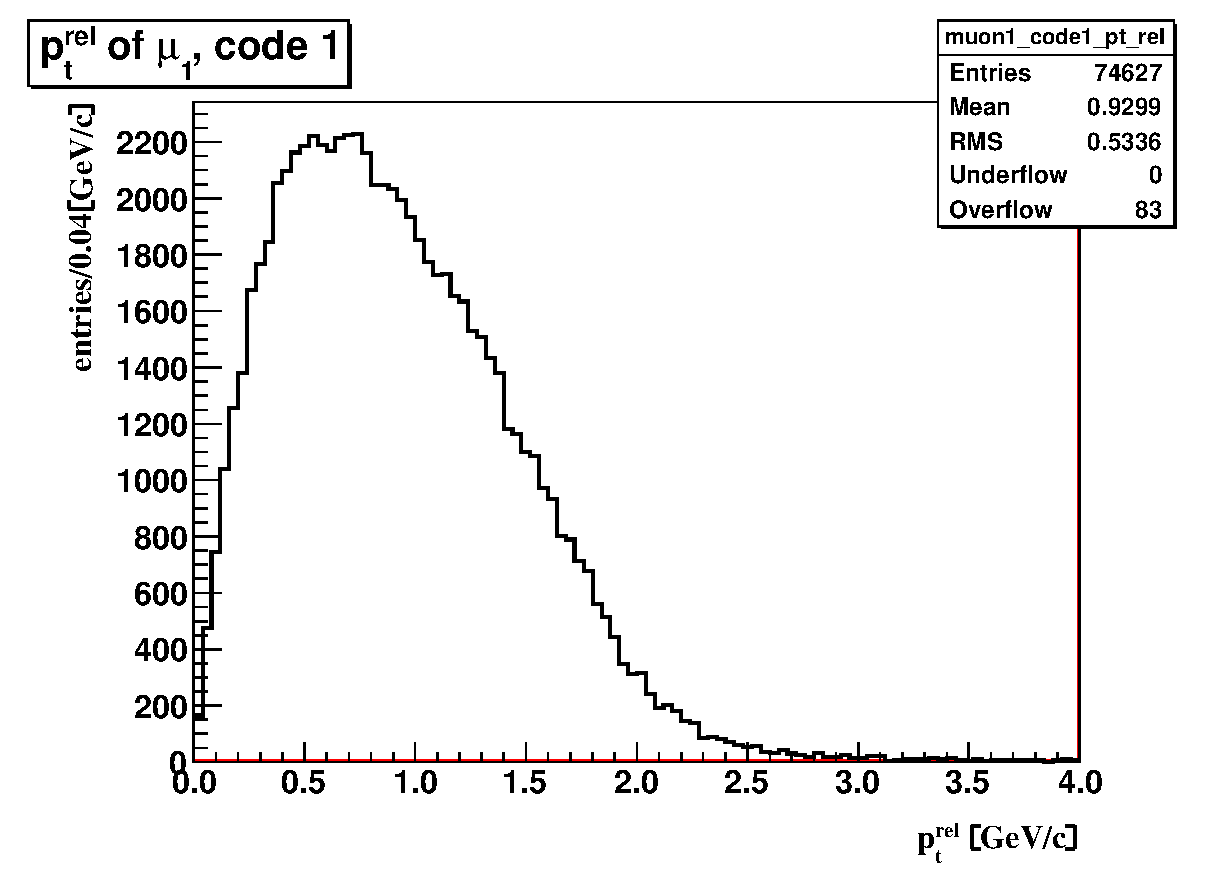
\includegraphics[width=\textwidth]{muon1_code1_pt_rel.eps}
            \end{figure}
        \end{column}
        \begin{column}{.5\textwidth}
            \centering
            fondo da $c$
            \begin{figure}[h]
                \centering
                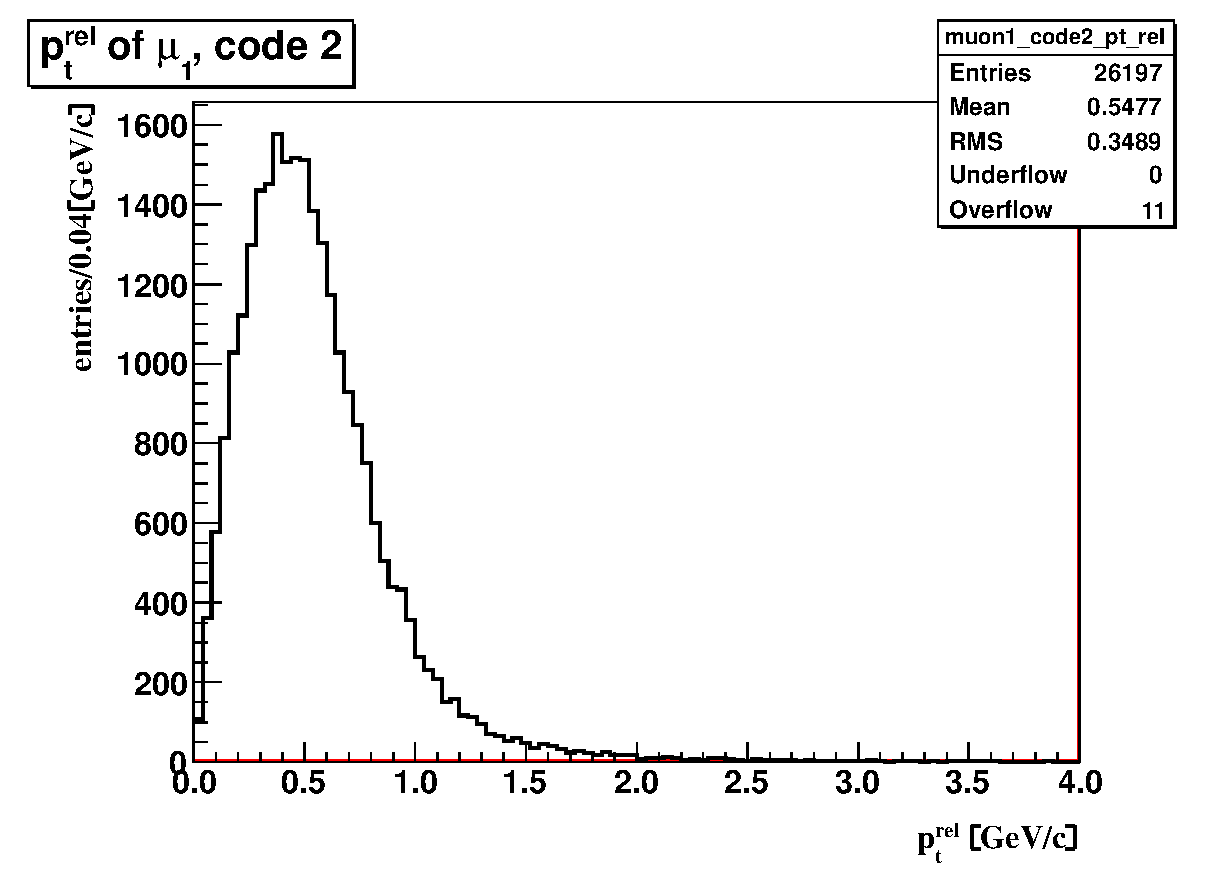
\includegraphics[width=\textwidth]{muon1_code2_pt_rel.eps}
            \end{figure}
        \end{column}
    \end{columns}
\end{frame}
\begin{frame}
    \frametitle{Distribuzioni in \ptrel{} dei dimuoni}
    \framesubtitle{Studio della correlazione}
    \begin{columns}
        \begin{column}{.5\textwidth}
            \begin{figure}[h]
                \centering
                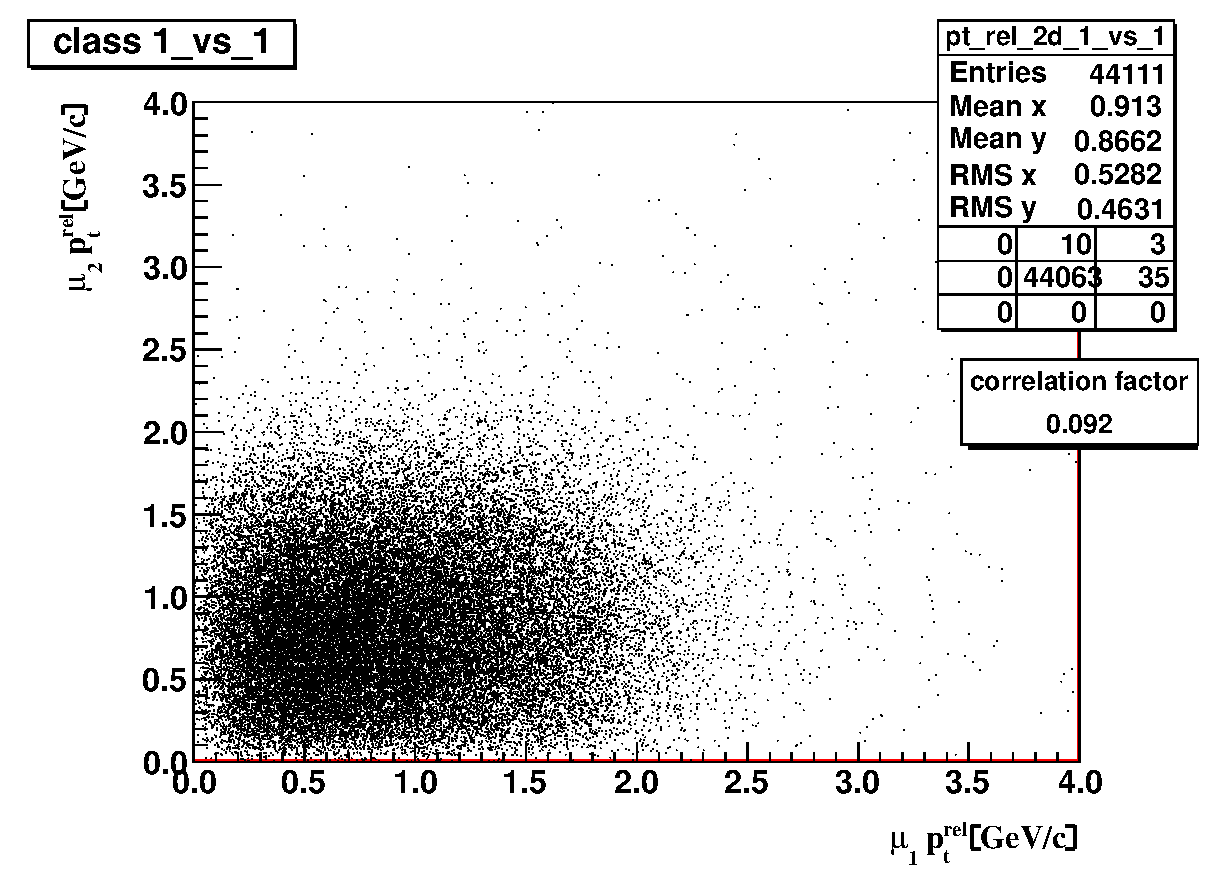
\includegraphics[width=.7\textwidth]{pt_rel_2d_1_vs_1.eps}
            \end{figure}
            \begin{figure}[h]
                \centering
                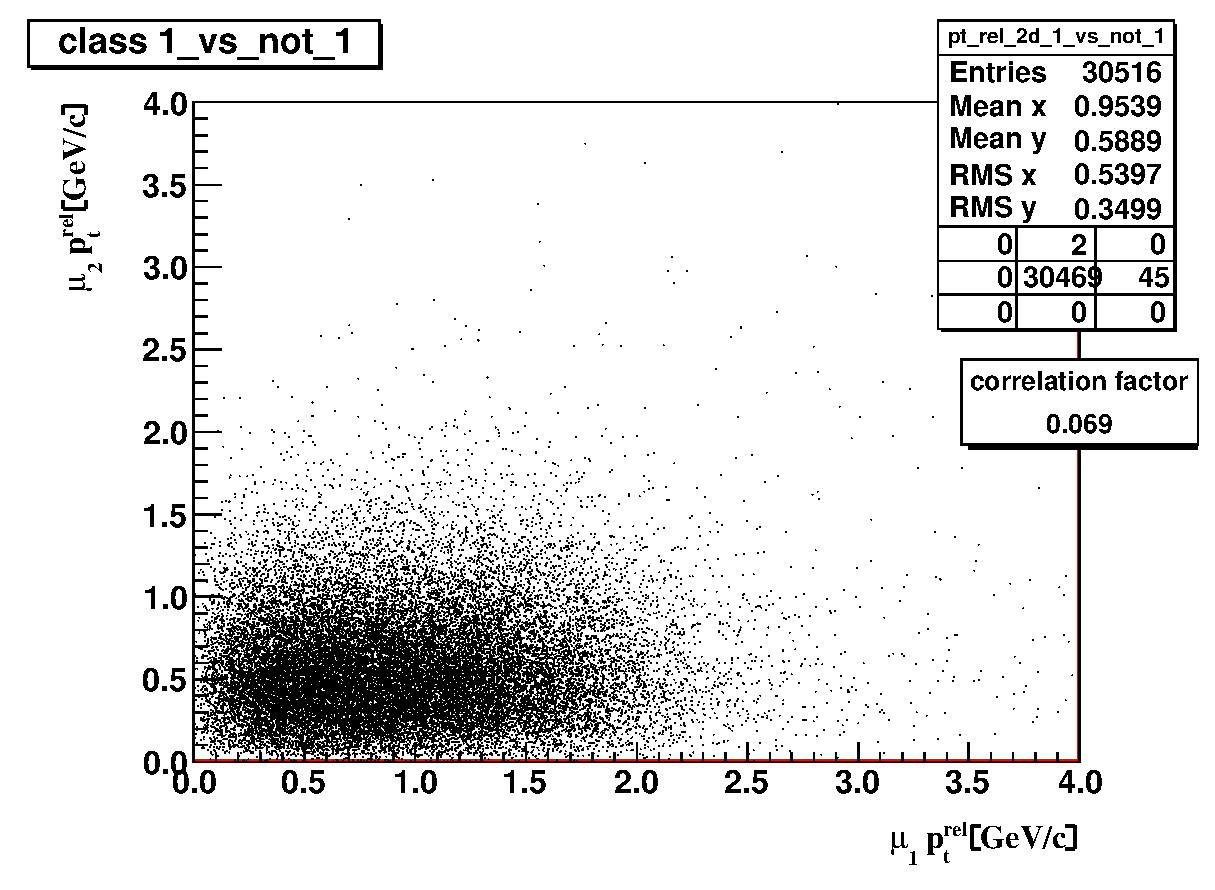
\includegraphics[width=.7\textwidth]{pt_rel_2d_1_vs_not_1.eps}
            \end{figure}
        \end{column}
        \begin{column}{.5\textwidth}
            \begin{figure}[h]
                \centering
                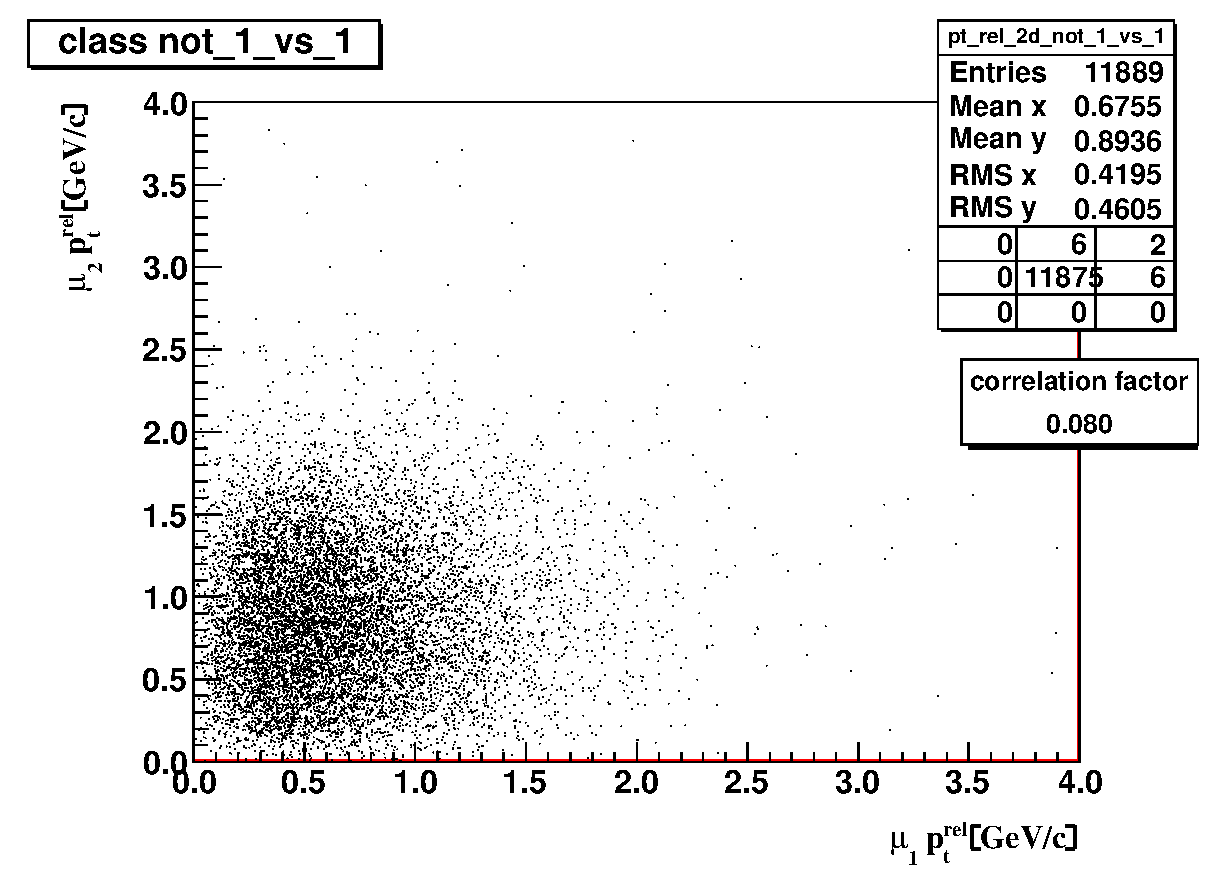
\includegraphics[width=.7\textwidth]{pt_rel_2d_not_1_vs_1.eps}
            \end{figure}
            \begin{figure}[h]
                \centering
                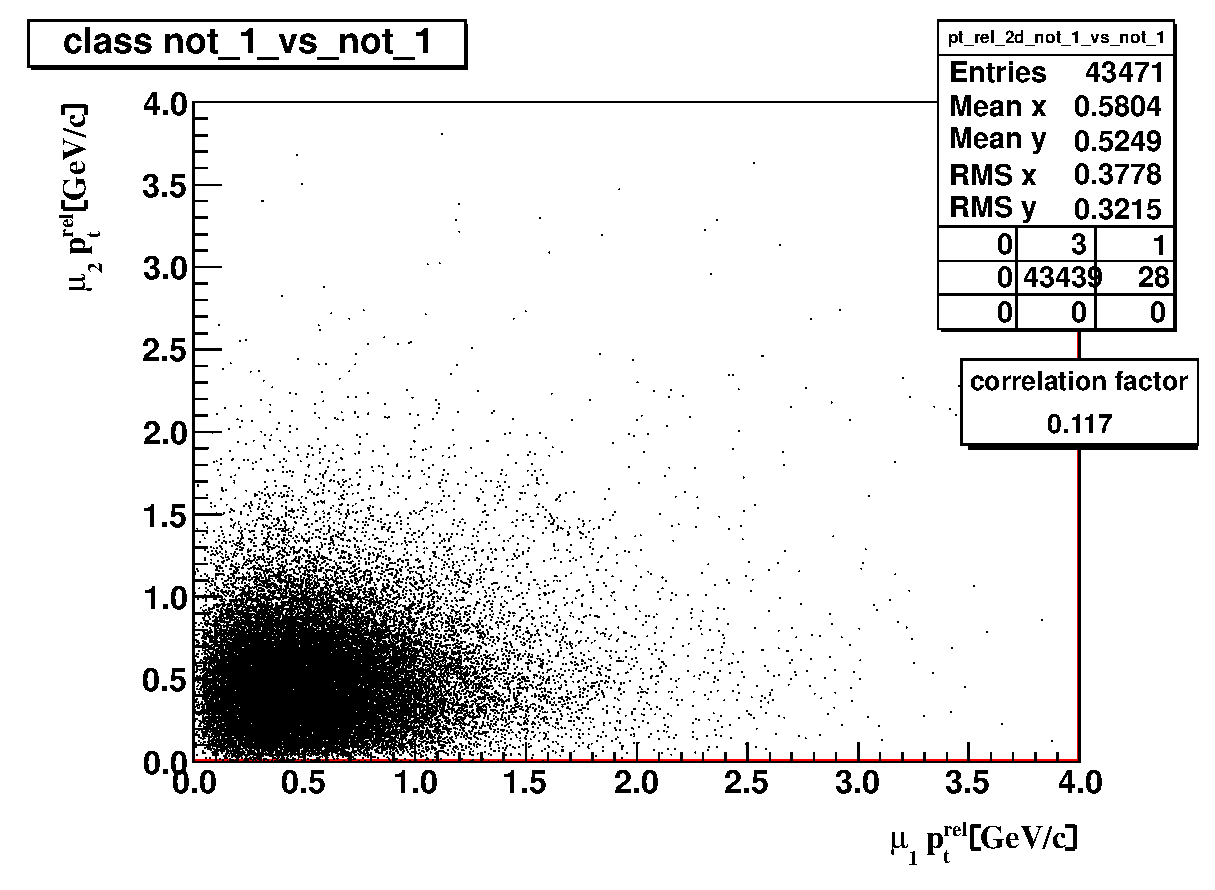
\includegraphics[width=.7\textwidth]{pt_rel_2d_not_1_vs_not_1.eps}
            \end{figure}
        \end{column}
    \end{columns}
\end{frame}
\begin{frame}
    \frametitle{Fit della distribuzione complessiva su MC}
    Divisione dei fondi nelle quattro distribuzioni della slide precedente.
    Fit delle frazioni.

    Risultati sul MC:
    \begin{table}
        \centering
        \begin{tabular}{r@{$\pm$}l c}
            \multicolumn{2}{c}{frazione fit} & frazione vera\\
            0.340 & 0.006 & 0.339\\
            0.234 & 0.005 & 0.234\\
            0.092 & 0.004 & 0.091\\
            0.335 & 0.005 & 0.333\\ 
        \end{tabular}
    \end{table}
\end{frame}
\begin{frame}
    \frametitle{Fit della distribuzione complessiva sui dati}
    \begin{block}
        {Difficoltà aggiuntiva}
        il campione di dati è più grande del campione MC.
    \end{block}
    Occorre aumentare la statistica.
    \vspace{2\baselineskip}\\
    \begin{columns}
        \begin{column}{.3\textwidth}
            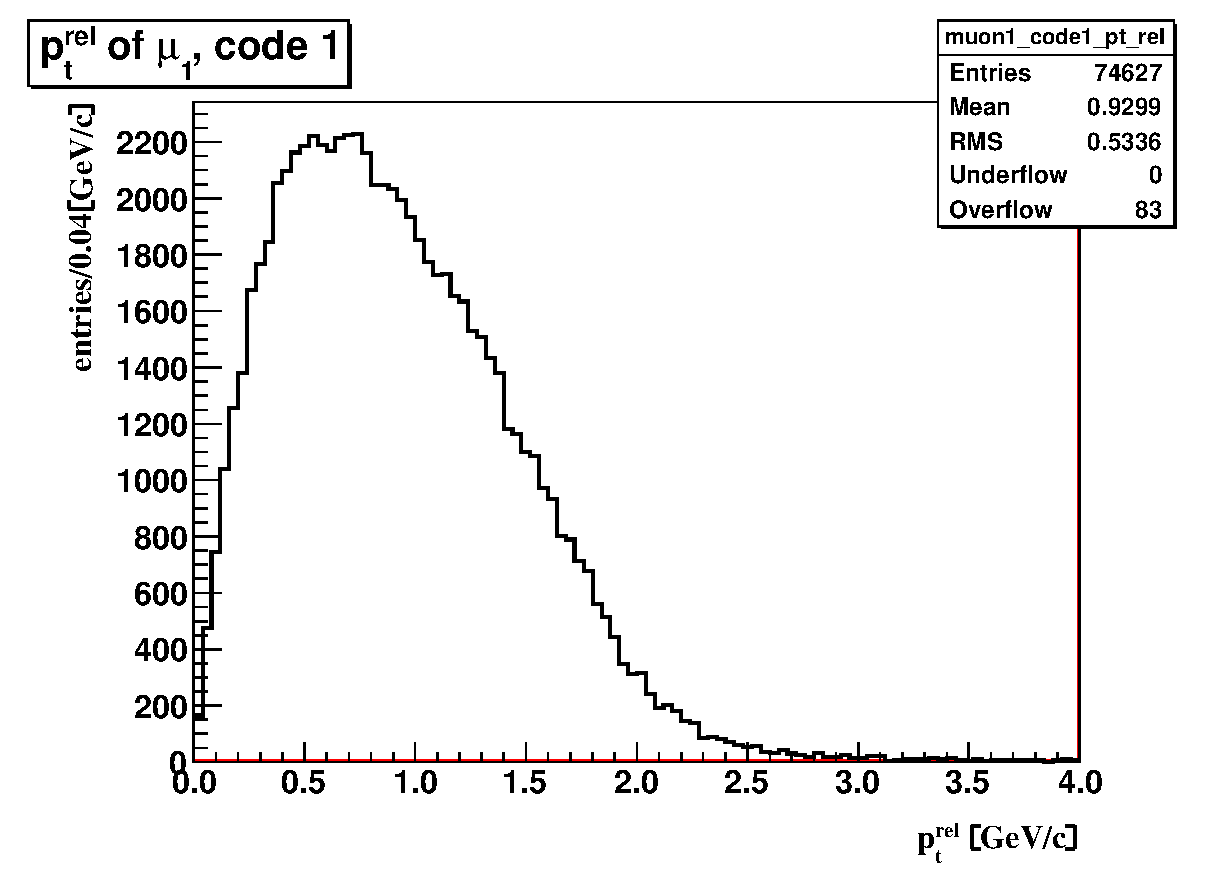
\includegraphics[width=.8\textwidth]{muon1_code1_pt_rel.eps}
            +
        \end{column}
        \begin{column}{.3\textwidth}
            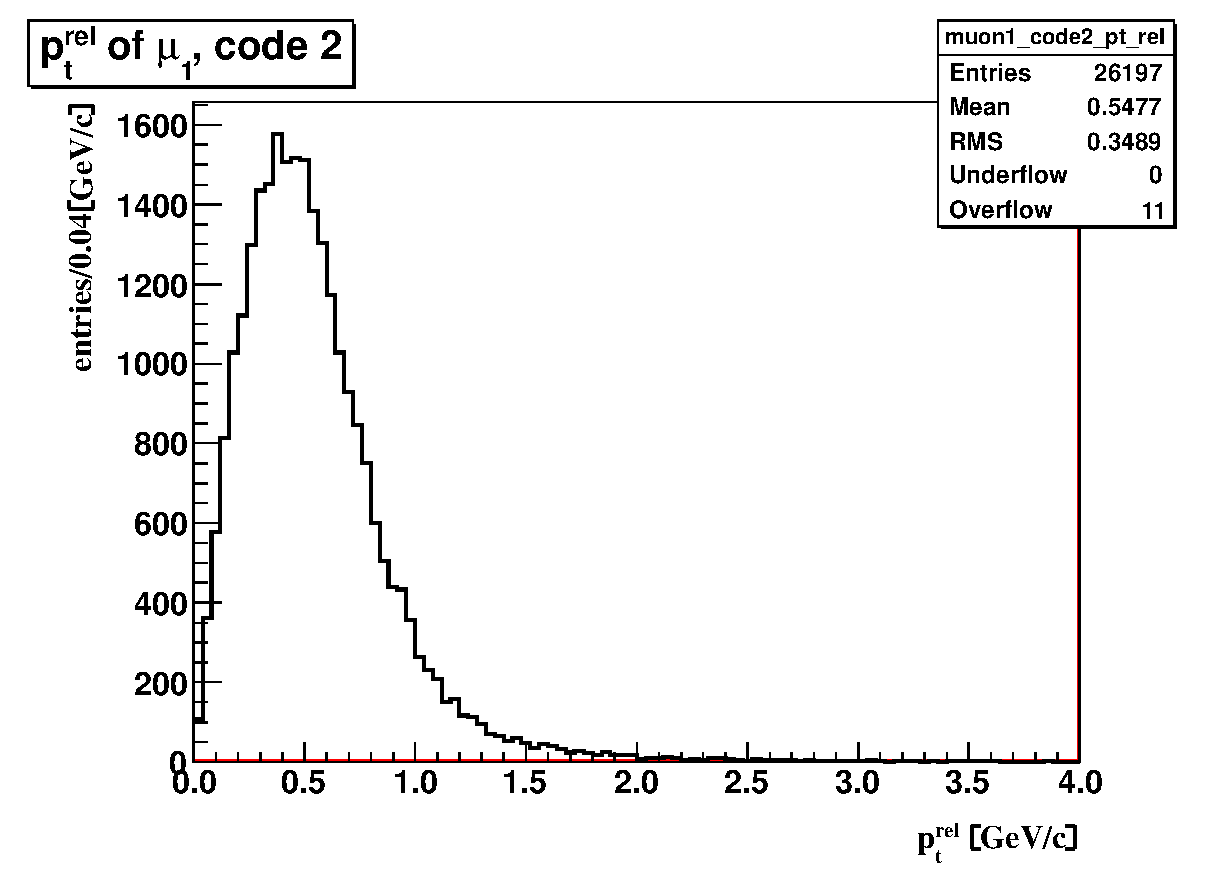
\includegraphics[width=.8\textwidth]{muon1_code2_pt_rel.eps}
            $\rightarrow$
        \end{column}
        \begin{column}{.3\textwidth}
            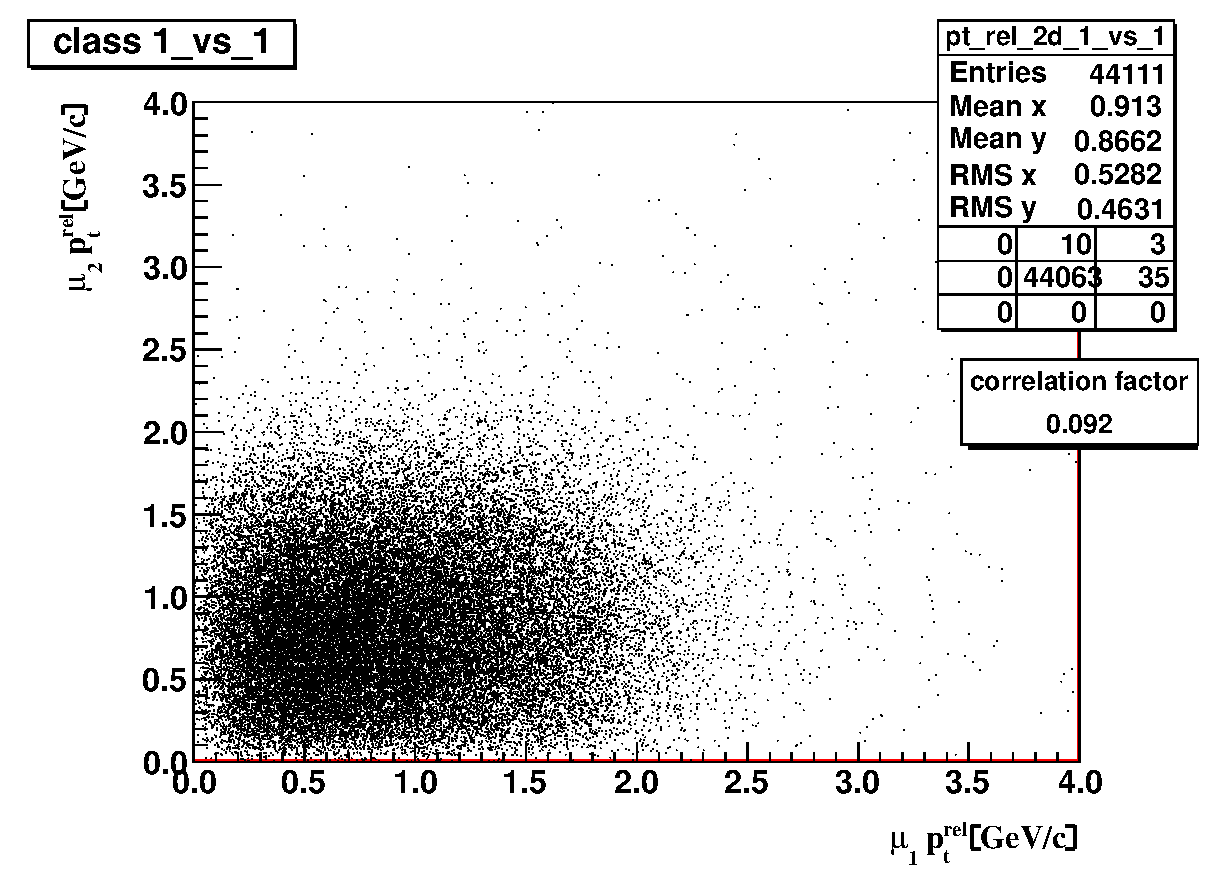
\includegraphics[width=.8\textwidth]{pt_rel_2d_1_vs_1.eps}
        \end{column}
    \end{columns}

    \vspace{2\baselineskip}
    \emph{template} con un milione di eventi ciascuno.

\end{frame}
\begin{frame}
    \frametitle{Fit della distribuzione complessiva sui dati}
    \framesubtitle{Risultati}
    \begin{columns}
        \begin{column}
            {.6\textwidth}
            \begin{figure}[h]
                \centering
                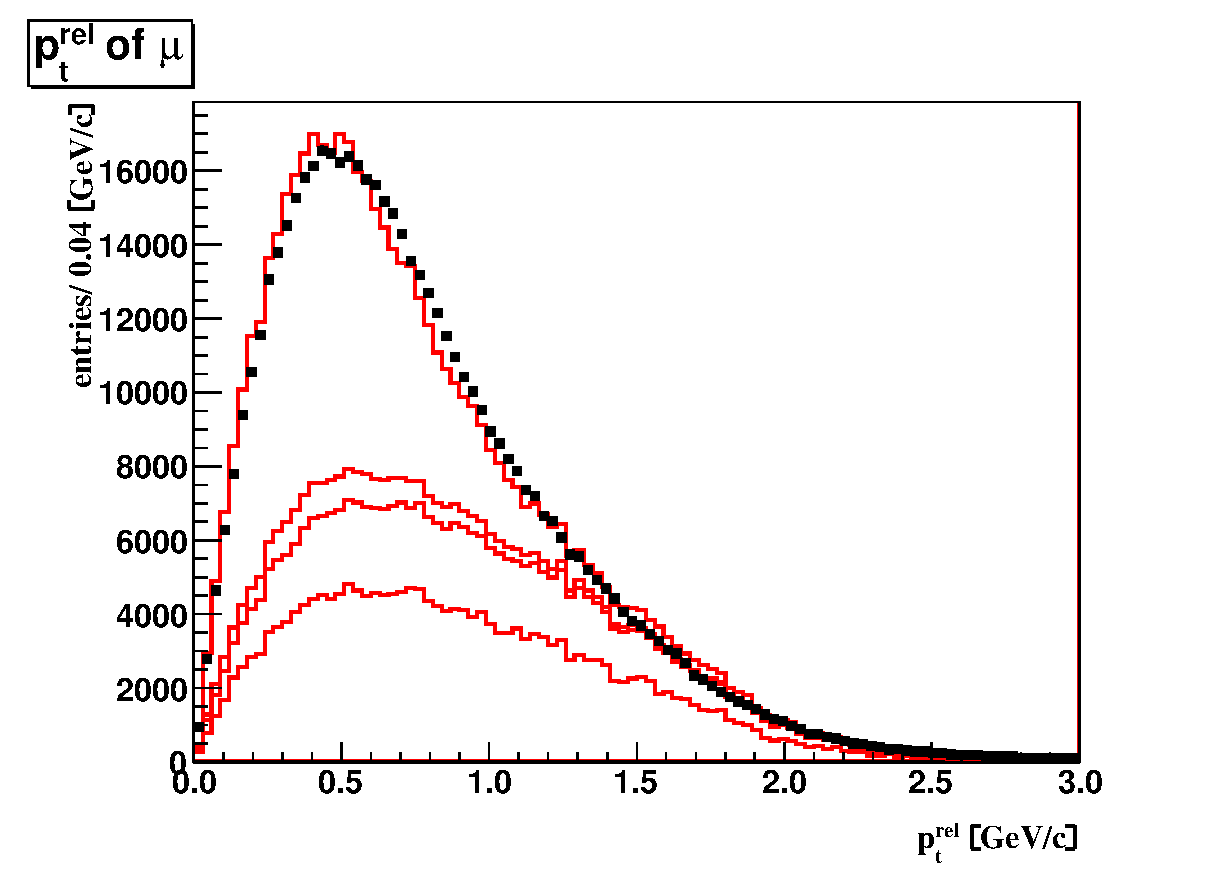
\includegraphics[width=\textwidth]{stack_fit.eps}
            \end{figure}
        \end{column}
        \begin{column}
            {.5\textwidth}
            \begin{table}
                \centering
                \begin{tabular}{r@{$\pm$}l c}
                    \multicolumn{2}{c}{frazione fit} & MC\\
                    0.360 & 0.004 & 0.339\\
                    0.192 & 0.003 & 0.234\\
                    0.047 & 0.003 & 0.091\\
                    0.400 & 0.002 & 0.333\\
                \end{tabular}
            \end{table}
        \end{column}
    \end{columns}

\end{frame}
\begin{frame}
    \frametitle{Conclusioni}
    \begin{itemize}
        \item la discriminazione con \ptrel{} funziona bene sul MC;
        \item ignorare la correlazione ($\sim 10\%$) nei dati produce un fit
            impreciso;
        \item è probabilmente necessario aumentare la statistica del MC
            all'origine;
    \end{itemize}
\end{frame}

\begin{frame}
    \frametitle{Backup slides}
\end{frame}

\begin{frame}
    \frametitle{Il rivelatore CMS}
    \begin{figure}[h]
        \begin{center}
            \includegraphics[width=.5\textwidth]{Schematic.eps}
        \end{center}
    \end{figure}
    \begin{description}
        \item[Tracker] cilindri concentrici di sensori al silicio. Misura
            l'impulso delle particelle cariche.
        \item[Calorimetri] misurano l'energia di elettroni e fotoni (ECAL) e
            di adroni (HCAL).
        \item[Rivelatori $\mu$] camere a deriva, solo i muoni sono abbastanza
            penetranti da raggiungerle.
    \end{description}
\end{frame}
\begin{frame}{Sistema di riferimento di CMS}
    \begin{itemize}
        \item pseudorapidità $\eta = -\log \tan
            \nicefrac{\theta}{2}$
        \item $\eta$ ha lo stesso segno di $z$ e va da $-\infty$ a
            $+\infty$
    \end{itemize}
    \begin{figure}[h]
        \begin{center}
            \psset{unit=1.15,viewpoint=2 1.5 1}
            \begin{pspicture}(0,0)(2.5,2.5)
                %xz plane
                \psset{arrows=->}
                \ThreeDput[normal=0 0 1]{
                \psline[linewidth=1pt]{}(0,0)(2, 1.154)
                \psarc{->}{1}{0}{30}
                \rput[l]{120}(1.35, 0.30){$\theta$}
                }      

                %zy plane
                \ThreeDput[normal=0 1 0]{
                \psline(0,0)(0,3)
                \psline(0,0)(-3,0)\uput[0](-3.5,0){$z$}
                \uput[0](-4.5,0.5){\small{direz. del fascio}}
                }      

                %xy plane
                \ThreeDput[normal=1 0 0]{
                \psline(0,0)(3,0)\uput[0](3,0){$x$}
                \uput[0](2.5,0.5){\small{centro di LHC}}
                \uput[0](0,3){$y$}
                \psline[linewidth=1pt]{}(0,0)(2,1.154)
                \psarc{->}{1}{0}{30}
                \uput[0](1.05,0.40){$\phi$}
                }      
            \end{pspicture}
        \end{center}
    \end{figure}
\end{frame}

\begin{frame}
    \frametitle{Distribuzione 2d dei dati}
    \begin{figure}[h]
        \centering
        \includegraphics[width=\textwidth]{muon_pt_rel_codes_999_vs_999.eps}
    \end{figure}
\end{frame}

\end{document}
